\chapter{Data Processing}
\label{sec:data_processing}

One of the most important aspects of the model development process is the data. The data is used to train the model and to evaluate the model. Therefore, it is important to ensure that the data is of high quality. During the development of the project, multiple different approaches were considered. First, $REPLACE_WE$ will discuss the different approaches that were considered and then $REPLACE_WE$ will discuss the approach that was chosen. $REPLACE_WE$ then discuss difficulties that were encountered during the data processing process.

As mentioned earlier, $REPLACE_WE$ propose a method that enables the fault detection of human pose estimation. Therefore, part of the data processing process is human pose estimation. In section \ref{sec:related_work}, $REPLACE_WE$ have already discussed different methods that can be used for human pose estimation. In the scope of this thesis, $REPLACE_WE$ will only focus on a single human pose estimator. This has multiple reasons. Firstly, $REPLACE_WE$ do not intend to develop a general fault detector. Different pose estimators have different flaws so increasing the pool of pose estimators would presumably create a more general fault detector but less accurate fault detector. Some faults might be generally applicable while others are more specific to a specific estimator. This is especially true if a pose estimator uses a different modality, e.g., OpenPose solely uses RGB data, whereas the human pose estimator proposed by C. Zimmermann et.al utilises RGBD data\cite{OpenPosePose, RGBDHPEforRoboticTaskLearning}. Furthermore, different pose estimators usually do not result in the same joints as they have been developed for different purposes. For example, OpenPose detects multiple joints in the face, while others use a single head joint. This discrepancy makes it difficult to develop a general fault detector for multiple pose estimators. 

We chose the same pose estimator that is used by SilverFit. SilverFit uses Nuitrack which was developed by 3DiVi Inc\footnote{\url{https://nuitrack.com/}}. Nuitrack does not offer any official white paper or mention how exactly their pose estimation works let alone which modality is used. On further inquiry, a representative notes that since around 2013 Nuitrack uses a similar technique as mentioned by J. Shotton et.al in their paper \textit{Real-time human pose recognition in parts from single depth images}\cite{EarlyRGBDHPE}. The method uses random forests to estimate the human pose. However, more recently Nuitrack has switched to Deep Learning with Convoluted Neural Networks, which is becoming more and more the industry standard for computer vision tasks such as human pose estimation.

\section{Data acquisition}
\label{sec:data_acquisition}

Different modalities were captured to create a dataset that reproduces a real-world application of HPE for RGB-D cameras. The different modalities are RGB data, depth data, and joint data. While the Nuitrack SDK offers to capture the data from the RGB-D cameras and the joint data, the recorded files cannot, at the time of writing, be read without using the Nuitrack SDK. Therefore, FESDData, a custom RGB-D+HPE capturing and labelling tool was developed. 

FESDData has two main uses which are interlocked. Firstly, it allows capturing predefined, as well as custom, exercises repeatedly automatically making the capturing experience when capturing many different exercises with multiple repetitions more comfortable. Secondly, it allows reviewing and labelling the captured data with error labels. The lightweight nature of FESDData allows it to seamlessly capture both the RGB-D stream and the skeleton data at the same time while ensuring a stable fast framerate. The dataset that is used by FESDModel was captured at a framerate of 30 frames per second. The interface of FESDData can be seen in figure \ref{fig:fesddata}. On the left side of the image the interface can be seen and on the right, there is an example for data labelling of Exercise E1-02.


\begin{figure}
  \centering
  \begin{subfigure}[b]{0.49\linewidth}
      \centering
      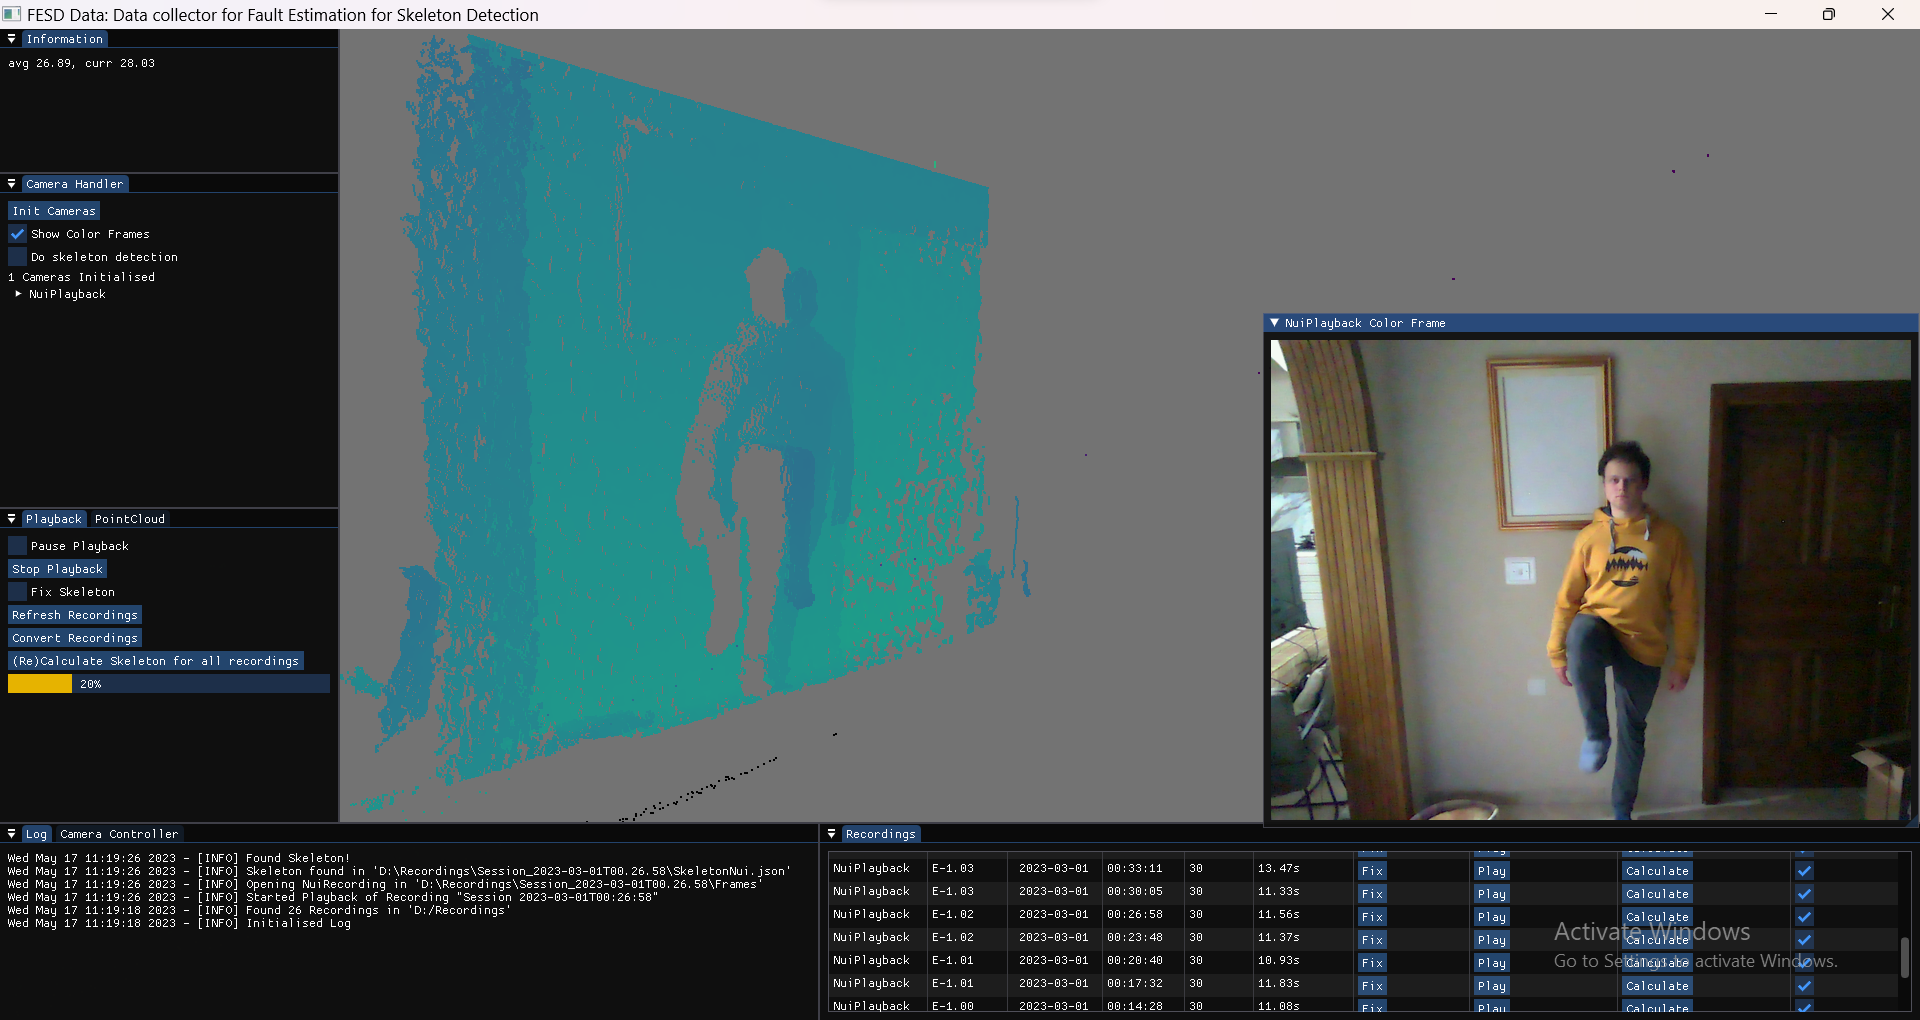
\includegraphics[width=\textwidth]{figures/FESDData/streaming.png}
  \end{subfigure}
  \hfill
  \begin{subfigure}[b]{0.49\linewidth}
      \centering
      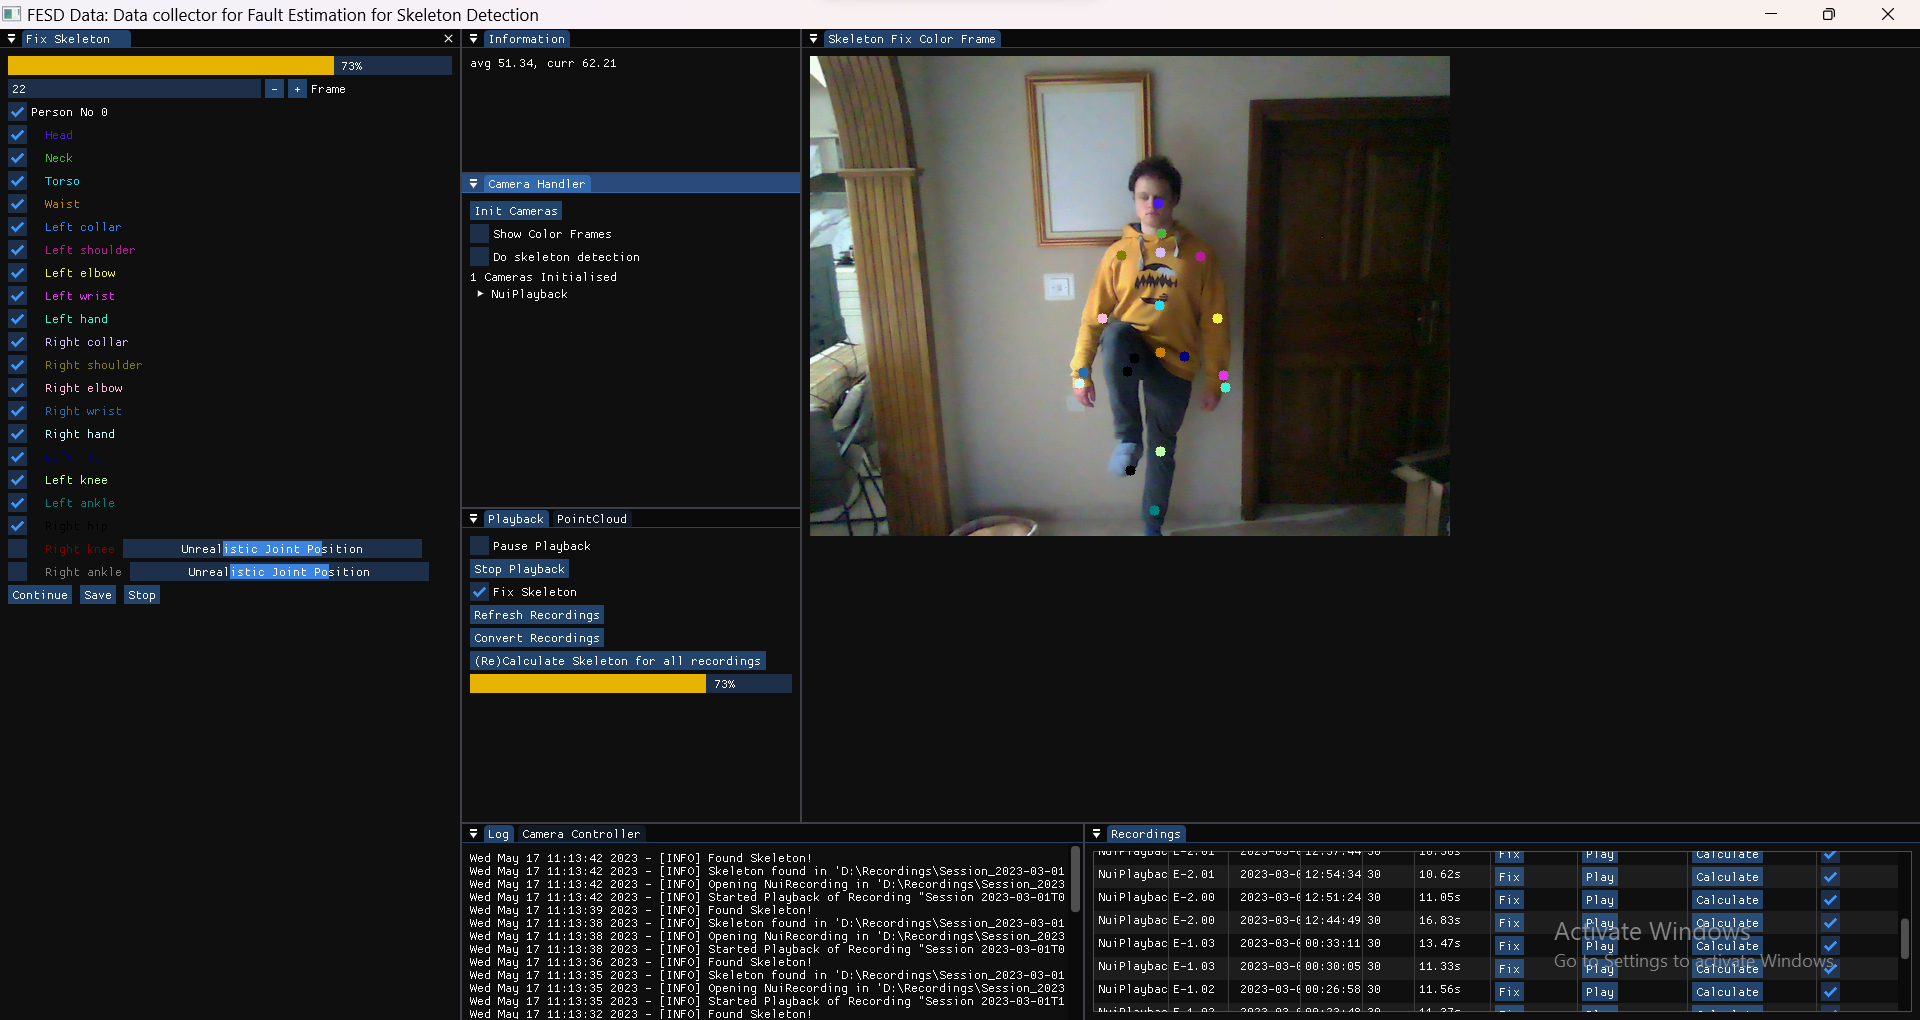
\includegraphics[width=\textwidth]{figures/FESDData/labelling.png}
  \end{subfigure}
  \caption[FESDData user interface]{A screenshot of the user interface with its two main components. On the left side, the user interface during streaming and recording can be seen and on the right side an example of data labelling.}
  \label{fig:fesddata}
\end{figure}  

\section{Data layout}

As mentioned earlier, the data is made up of multiple different streams or modalities. There are two separate visual streams, the RGB stream, and the depth stream, as well as the estimated human pose, the time stamps, and the recording metadata.

The visual streams are normalised and combined into a single file. OpenCV is used to store the RGB and the depth data into a single matrix and after the stream into a single file per frame. The RGB data is normalised to have values between 0 and 1, whereas the depth data is stored in meters.

The pose that is estimated by Nuitrack, as well as the error labels, are stored in a separate JSON file. The separate frames are stored in a list of frames. Each frame contains a list of all people that were detected. Each person contains a list of joints as well as an error label. Each joint is stored with real-world 3D coordinates which are stored in meters. These real-world coordinates are labelled $x$, $y$, and $z$. Additionally, the 2D projection and depth of the joint are stored in image coordinates and meters for the depth. The 2D projection is labelled $u$ and $v$ and the depth is labelled $d$. 

The error label is an integer which is the error id specific for joint and skeleton errors. The errors corresponding to the error ids are explained in section \ref{sec:data_labeling}. Finally, the timestamp of each frame is stored.

\subsection{Data labeling}
\label{sec:data_labeling}

A large part of the data preparation is the labelling of the data. The data is labelled with error labels. We define two different areas of errors. First, there are skeleton errors. Skeleton errors occur when the pose estimator detects a human in places where there are no humans. This can be caused by the pose estimator detecting a human in the background due to certain features that the estimator assumes are human.

Second, there are joint errors. Joint errors occur when the pose estimator detects a joint in the wrong place. This can be caused by the pose estimator detecting a joint in the background due to certain features that the estimator assumes are a joint. It can also be caused by the estimator labelling a joint incorrectly. 

For example, the estimator might label the left foot as the right foot. This is a common error, especially when the limbs are close too each other. An estimator might also not detect a joint at all. This might be caused through occlusion, be it by another joint, an object, or by the image border. Most applications avoid the last cause for occlusion by defining a minimum distance from the camera and specific camera placement to ensure that the user is always fully in view.

In the data, no error is denoted with $0$. If the whole skeleton is in a wrong position it can be labeled as faulty and subsequently every joint will be labeled with $2$. If a joint is not detected at all, it is labelled with $1$. If a joint is detected in the wrong place that is outside of the body, or somewhere where there should not be a joint, it is labelled with $2$. If a joint is detected in the approximate position of where another joint should be then it is labelled with $3$.

Implicitly, this creates two general labels, either a joint is faulty, i.e. the error label is $1$, $2$, or $3$, or it is not faulty, i.e. the error label is $0$. This makes the task easier, as it is a binary classification rather than a multi-class classification. However, we find the result to be enlightening as they might be more accurate and therefore more reliable.
\section{Dataset}

Multiple iterations of the recording process were run to find the best possible setup, which reduces the light interference as much as possible and which offers the best results with the resources at hand. The camera setup that is used by SilverFit was reproduced. At SilverFit the camera is mounted at $175cm$ above the floor. The camera that is used has an accelerometer which was used to adjust the camera angle relative to the ground. The camera is angled downward at a $70^\circ$ angle. 



% \subsection{Analysis}

% An important aspect of the dataset is the structure and distribution of data and their labels. In total, $REPLACE_WE$ recorded all 13 exercises, mentioned in Section \ref{sec:exercises}, twice. Each recording session consists of exactly 300 frames.

% If a joint cannot be detected by Nuitrack it automatically gets zero coordinates, i.e. every value is zero. This makes it easy to automatically label these joints as faulty, in particular with the error label $1$ - Joint Missing. However, for the rest of the errors each frame has to be manually inspected and each joint considered. Since this requires a lot of work $REPLACE_WE$ reduced the labeled frames to 10 percent of the original size. Therefore, each exercise contains 30 frames and in total $30 \cdot 13 \cdot 2 = 720$ frames are labeled.

% When multiple persons are detected one person might be incorrectly detected in the background. While analysing the data $REPLACE_WE$ pick the person that is not labeled as faulty whenever possible. For training and testing this is chosen at random. If a person is labeled as faulty each joint is marked as in an unrealistic position.

% \subsubsection{Distribution of Errors}

% An important factor in how well a model can be trained on data is the balance of the dataset. In this case, the dataset is balanced by the error labels. In Figure \ref{fig:statistics_err_dist} $REPLACE_WE$ can see the distribution of errors in the dataset as a whole. $REPLACE_WE$ see that most of the joints are not faulty, i.e. are in the position they are supposed be within a margin of error.

% \begin{figure}
%   \centering
%   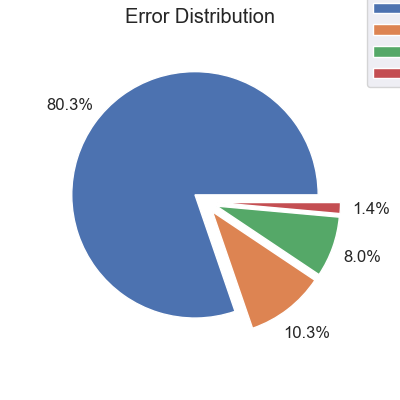
\includegraphics[width=0.5\textwidth]{figures/Data/Error_Distribution.png}
%   \caption[Error Distribution]{The distribution of errors TODO}
%   \label{fig:statistics_err_dist}
% \end{figure}

% To diversify the dataset $REPLACE_WE$ recorded different exercises with varying difficulties. In Figure \ref{fig:statistics_err_diff} $REPLACE_WE$ see that the difficulty has an influence on the amount of errors that occur for any given joint. $REPLACE_WE$ see that there is barely any difference between the trivial and the easy exercises. However, in Figure \ref{fig:statistics_err_dist_diff} $REPLACE_WE$ see that while trivial exercises have a higher percentage of unrealistic joint positions, i.e. the joint is in a wrong location, the easy exercises have a higher percentage of joints which are not detected. However, this difference is very small. Medium and Hard exercises are more error prone as was intended. This reflects $REPLACE_OUR$ design proposals for challenging exercises from Section \ref{sec:exercises} indeed cause more difficult scenarios.

% \begin{figure}
%   \centering
%   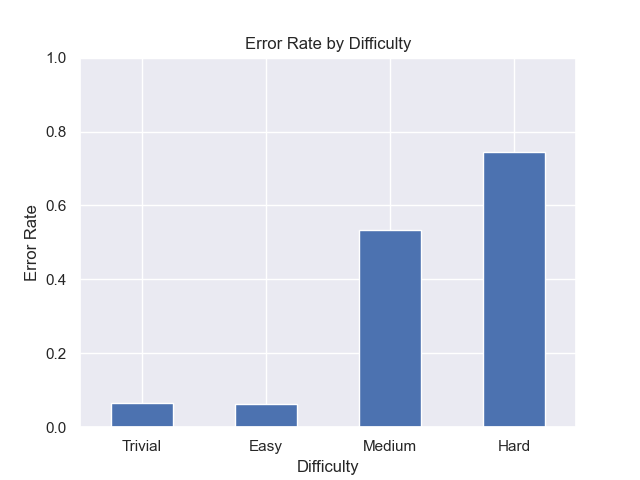
\includegraphics[width=0.5\textwidth]{figures/Data/Error_Rate_by_Difficulty.png}
%   \caption[Error Rate by Difficulty]{The rate that errors occur for any given difficulty. }
%   \label{fig:statistics_err_diff}
% \end{figure}

% \begin{figure}
%   \centering
%   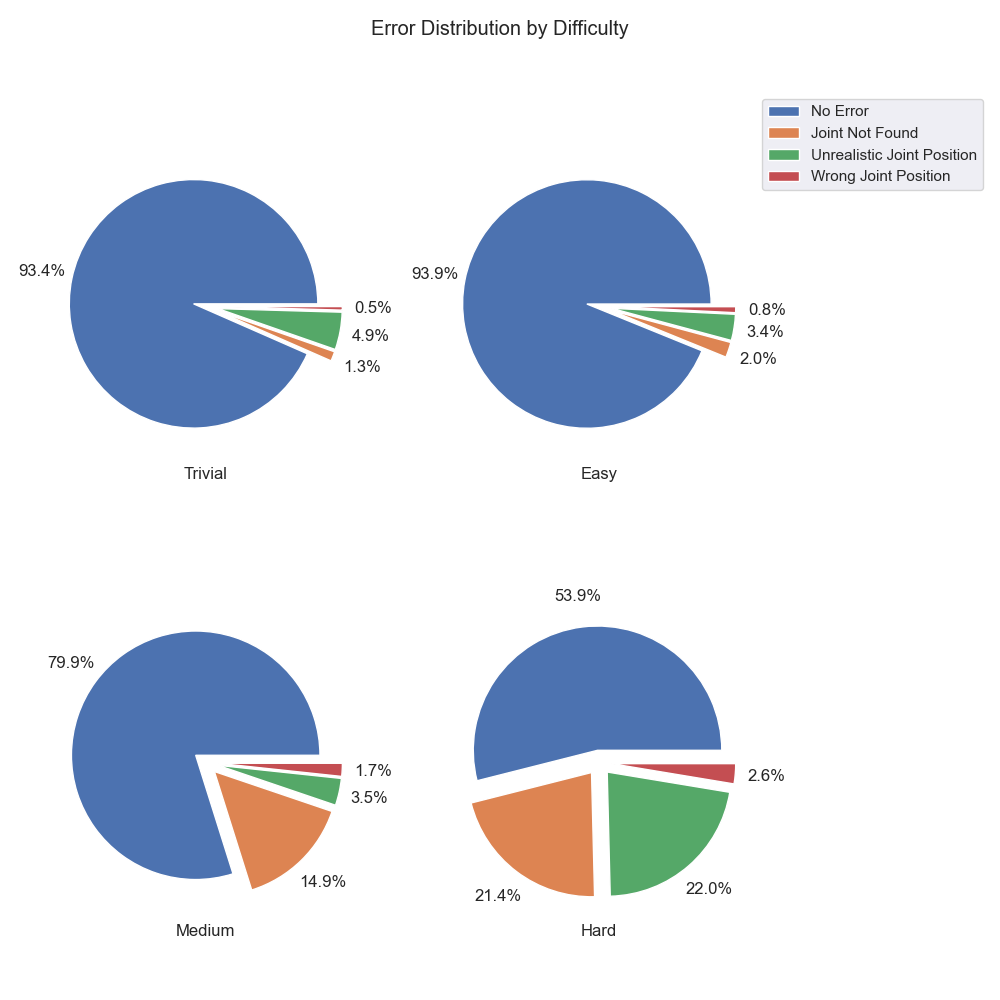
\includegraphics[width=0.5\textwidth]{figures/Data/Error_Distribution_by_Difficulty.png}
%   \caption[Error Distribution by Difficulty]{The distribution of errors by difficulty. TODO}
%   \label{fig:statistics_err_dist_diff}
% \end{figure}

% Some joints are more likely than others to be faulty, based on frequent occlusion, or generally more challenging detection. For example, hands and ankles are quite challenging to detect since they move frequently and are frequently occluded. On the other hand the head and the neck are least likely to be faulty. This distribution can be seen in Figure \ref{fig:statistics_err_dist_joint}, where the distribution of errors are shown for each joint. The joints are sorted by general occurrence of errors.

% \begin{figure}
%   \centering
%   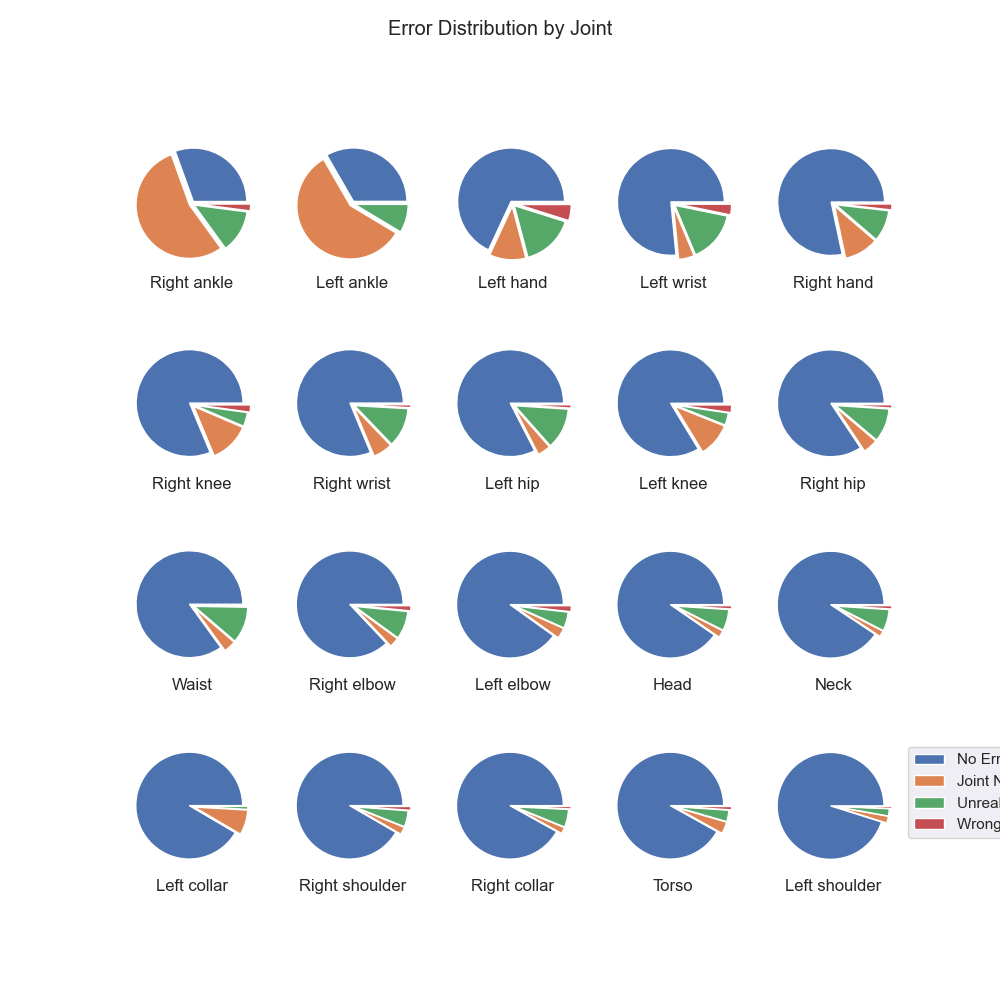
\includegraphics[width=0.5\textwidth]{figures/Data/Error_Distribution_by_Joint.png}
%   \caption[Error Distribution by Joint]{The distribution of errors by Joint. TODO}
%   \label{fig:statistics_err_dist_joint}
% \end{figure}

\subsection{Problem Sets}
\label{sec:problem_set}

Different problem sets are used to create different versions of the model. The problem sets are defined by the number of objects that are considered and are defined as erroneous. There are four different problem sets. The first problem set is the \textit{Joint} problem set. In this problem set, each joint is considered as a single object. The first simplification is to consider each joint, i.e. the individual arms, legs, torso, and head. The second simplification is to consider the upper and the lower body. Finally, only the whole body is considered.